\chapter{Produktudvikling}\label{Produktudvikling} 
Her beskrives 

\section{Systemarkitektur}\label{Systemarkitektur}
Der er udarbejdet forskellige diagrammer på baggrund af de specificerede systemkrav. Diagrammerne har til formål at dele systemet op i realiserbare dele for at vise arkitekturen for og designet af Automatisk Ultralydsscanner. 

Arkitekturen beskriver den grundlæggende organisering af Automatisk Ultralydsscanner og opbygningen af dens tilhørende PC Applikation. Der er i diagrammerne designet ud fra, at 3D kamera er af typen Microsoft Kinect 2.0 og Robotarm er en Universal Robot UR10 robot. 

Nedenfor vil relevante diagrammer blive gennemgået. For detaljeret gennemgang af systemarkitektur for Automatisk Ultralydsscanner se Bilag  \ref{Udviklingsdokument} Udviklingsdokument

\subsection{Domænemodel}
Nedenstående domænemodel Figur \ref{domain} udgør den overordnede systemarkitektur og tydeliggør forbindelserne samt interaktionerne mellem de forskellige aktører i Automatisk Ultralydsscanner. 

\begin{figure}[H]
    \centering
    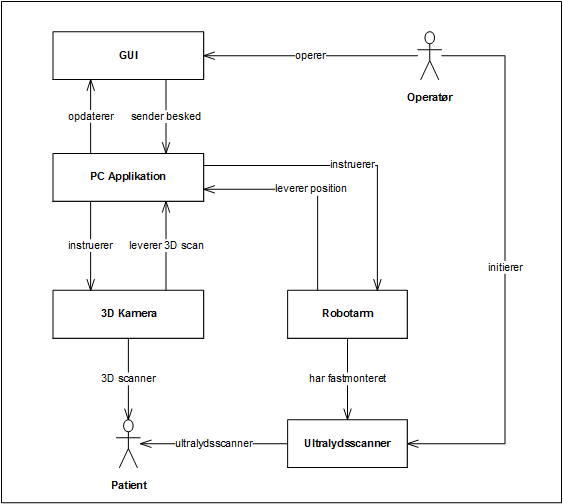
\includegraphics[width=0.7\textwidth]{figurer/d/Design/uml_domain}
    \caption{Domænemodel for Automatisk Ultralydsscanner}
    \label{domain}
\end{figure}

\subsection{Block definition diagram}
Automatisk Ultralydsscanner består af Robotarm, en computer, et Access Point, 3D kamera og Ultralydsscanner. Det er vigtigt at bemærke, at computer skal have PC Applikationen installeret og en mus og en skærm for at Operatør kan intergere med PC Applikation. Block Definitions diagrammet viser Figur \ref{BDD}, hvordan systemets blokke er forbundet. 

\begin{figure}[H]
    \centering
    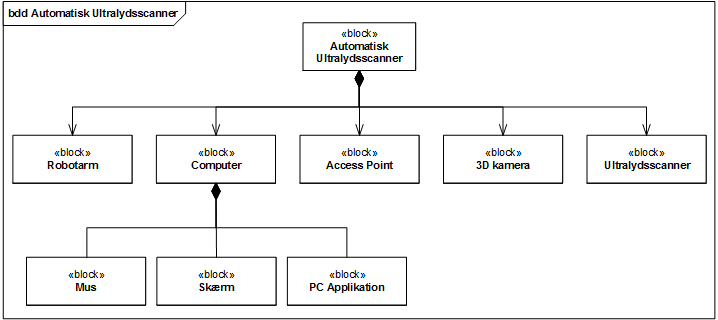
\includegraphics[width=1\textwidth]{figurer/d/Design/BDD}
    \caption{BDD for Automatisk Ultralydsscanner}
    \label{BDD}
\end{figure}

\subsection{Internal block diagram}
Detaljerne mellem interaktionen mellem de enkelte blokke er beskrevet i internal block diagram Figur \ref{IBD}, som viser systemets interne forbindelser og flow mellem de forskellige blokke. Bemærk at Ultralydsscanner ikke er inkluderet, da den ikke har forbindelse til de andre blokke udover at være fysisk monteret på robotarm. 

\begin{figure}[H]
    \centering
    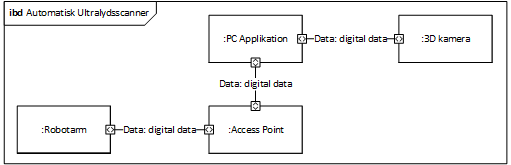
\includegraphics[width=1\textwidth]{figurer/d/Design/IBD}
    \caption{IBD for Automatisk Ultralydsscanner}
    \label{IBD}
\end{figure}

\subsection{Pakkediagram} 









\section{Systemdesign} \label{Systemdesign}
Systemdesignet beskriver hvordan PC Applikation er opbygget og hvordan PC Apllikations klasser integrerer med hinanden.  

Nedenfor vil relevante diagrammer blive gennemgået. For detaljeret gennemgang af systemdesign for Automatisk Ultralydsscanner se Bilag  \ref{Udviklingsdokument} Udviklingsdokument.

\subsubsection{Klassediagram}
Klassediagrammerne viser strukturen i systemet og deres relationer. Hver klasse indeholder de vigtigste metoder og attributer i klassen, der udgør funktionaliteten i PC Applikation. 

\subsubsubsection{GUI}
GUI-klassen Figur \ref{class_gui} indeholder brugergrænsefladen for PC Applikation.

\let\labelitemi\labelitemii
\begin{itemize}
\item{MainWindow}\newline
Giver anledning til at foretage et 3D scan. Såfremt en 3D scanning er gennemført giver det også anledning til at starte en ultralydsscanning.
Når menuen startes, oprettes en instans af RoboMaster, for at sætte Robotarm i standard positur. Dette er nødvendigt, hvis Robotarm skulle være i vejen for en 3D scanning.
Hvis der ikke er nogen forbindelse til Robotarm vil der 

\item{3DScanMenu}\newline
I denne menu er der mulighed for at se det nuværende dybdebillede, afgrænse området der skal 3D scannes og foretage en 3D scanning.

\item{UltrasoundScanMenu}\newline
I denne menu kan den procentvise færdiggørelse af ultralydsscanningen følges. Der er også mulighed for at pause samt afbryde ultralydsscanningsprocessen.
\end{itemize}

\begin{figure}[H]
    \centering
    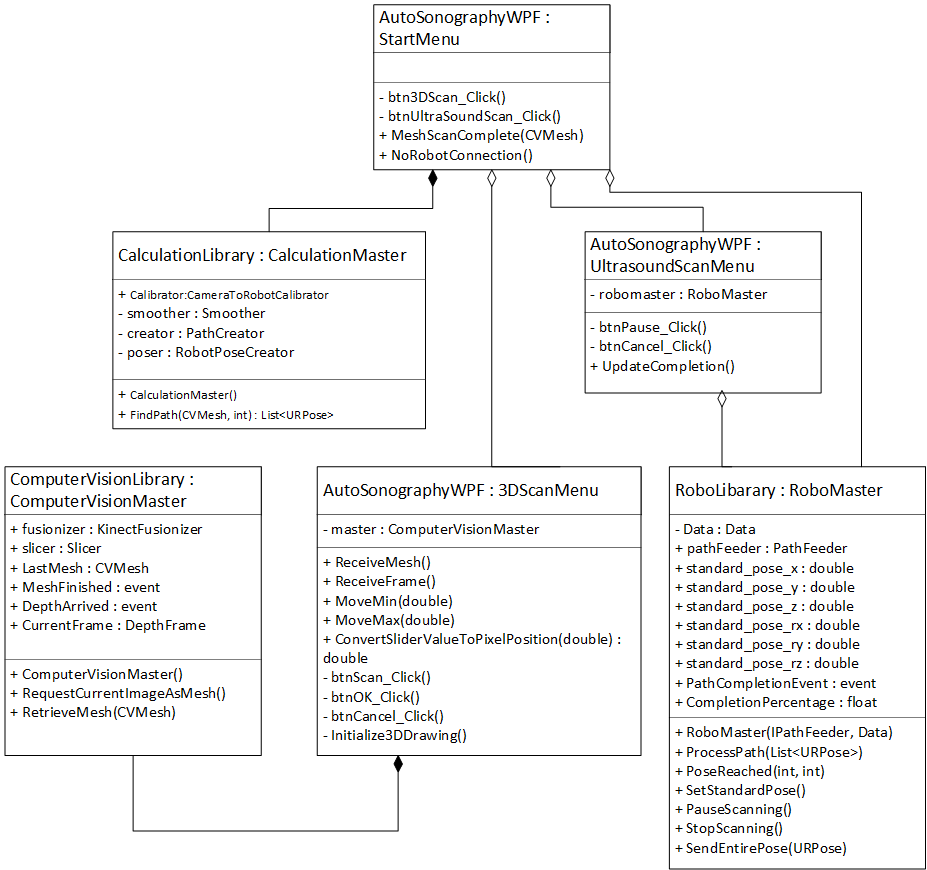
\includegraphics[width=1\textwidth]{figurer/d/Design/Class/uml_class_gui}
    \caption{Klassediagram for GUI}
    \label{class_gui}
\end{figure}

\subsection{Systemets grænseflader}


\section{Udviklingsmiljø} 



